\documentclass{beamer}
\mode<presentation>
\usepackage{ICES_beamer_template}
\usepackage[english]{babel}
\usepackage[utf8x]{inputenc}
\usepackage{amsmath,bm}

%===============================================================================
% 					  Presentation Title and Author  
%===============================================================================
\title[Updates]{Updates: Parameter Estimation}
\author{Xoab Perez}
\date{\today}

\begin{document}

\begin{frame}
  \titlepage
\end{frame}

% Uncomment these lines for an automatically generated outline.
%\begin{frame}{Outline}
% \tableofcontents
%\end{frame}

%===============================================================================
% Section 1
\section{Notes for Last Week}
%==================================================
\begin{frame}{Work done}
	\begin{minipage}[T][.7\textheight][t]{\textwidth}
		\begin{itemize}
			\item I spent some time last week computationally approximating bounds under which the nonlinear solver for hyperelasticity would converge (later, with more time, I can try to do this numerically) which led me to try parameter estimation with the following:
			\begin{align*}
			 k &\in [0,10] \\
			 D &\in [0,5] \\
			 \gamma_D &\in [.01,5] \\
			 \gamma_k &\in [.01,5] \\
			 \beta &\in [0.1,5] 
			 \end{align*}
			\item The bounds were not necessary for linear elasticity or reaction diffusion, but I kept them the same for the LE inverse problem for uniformity
		\end{itemize}
	\end{minipage}
\end{frame}

\begin{frame}{Work done}
	\begin{minipage}[T][.7\textheight][t]{\textwidth}
		\begin{itemize}
			\item I then worked on estimating parameters with these bounds in place. I was experimenting with different cost functions, and I only have results for minimizing difference in cellularity for now:
			\[ \min_{D,k,\gamma_D,\gamma_k,\beta} ||p_{true}-p||^2 \]
			\item I currently have optimized for rat 5 at day 2, then run the forward problem until the last day of data, day 9. 
		\end{itemize}
	\end{minipage}
\end{frame}

%===============================================================================
% Section2
\section{Results}
%==================================================
\begin{frame}{Results: Optimization for day 2}
	\begin{minipage}[T][.7\textheight][t]{.49\textwidth}
		LE
		\begin{itemize}
			\item Time = 14.5 minutes
			\item J-opt = 0.9
			\item $\gamma_D$ = .56
			\item $\gamma_k$ = 4.67
			\item $\beta$ = .96 
		\end{itemize}
	\end{minipage}
	\begin{minipage}[T][.7\textheight][t]{.49\textwidth}
		HE
		\begin{itemize}
			\item Time = 28 minutes 
			\item J-opt = 0.108
			\item $\gamma_D$ = .05
			\item $\gamma_k$ = 2.35
			\item $\beta$ = 4.0 
		\end{itemize}
	\end{minipage}
\end{frame}

\begin{frame}{Results: Optimization for day 2}
	\begin{figure}
    	\centering
    	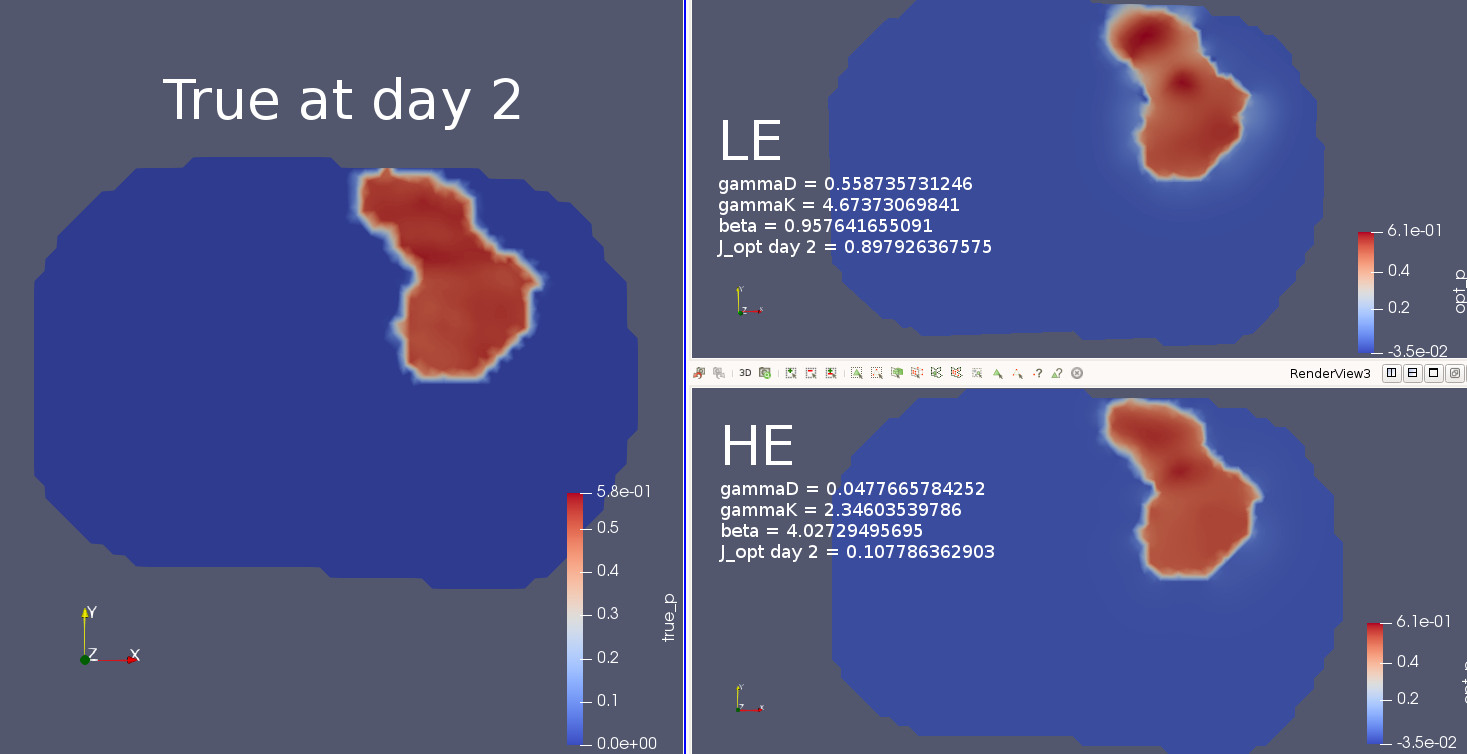
\includegraphics[width=\textwidth]{opt_day2.jpg}    	
    	\caption{Running the forward models to day 2 using parameter estimation results from forward model with day 2. Results for HE are better.}
    	\end{figure}	
\end{frame}

\begin{frame}{Results: Forward to day 6}
	\begin{figure}
    	\centering
    	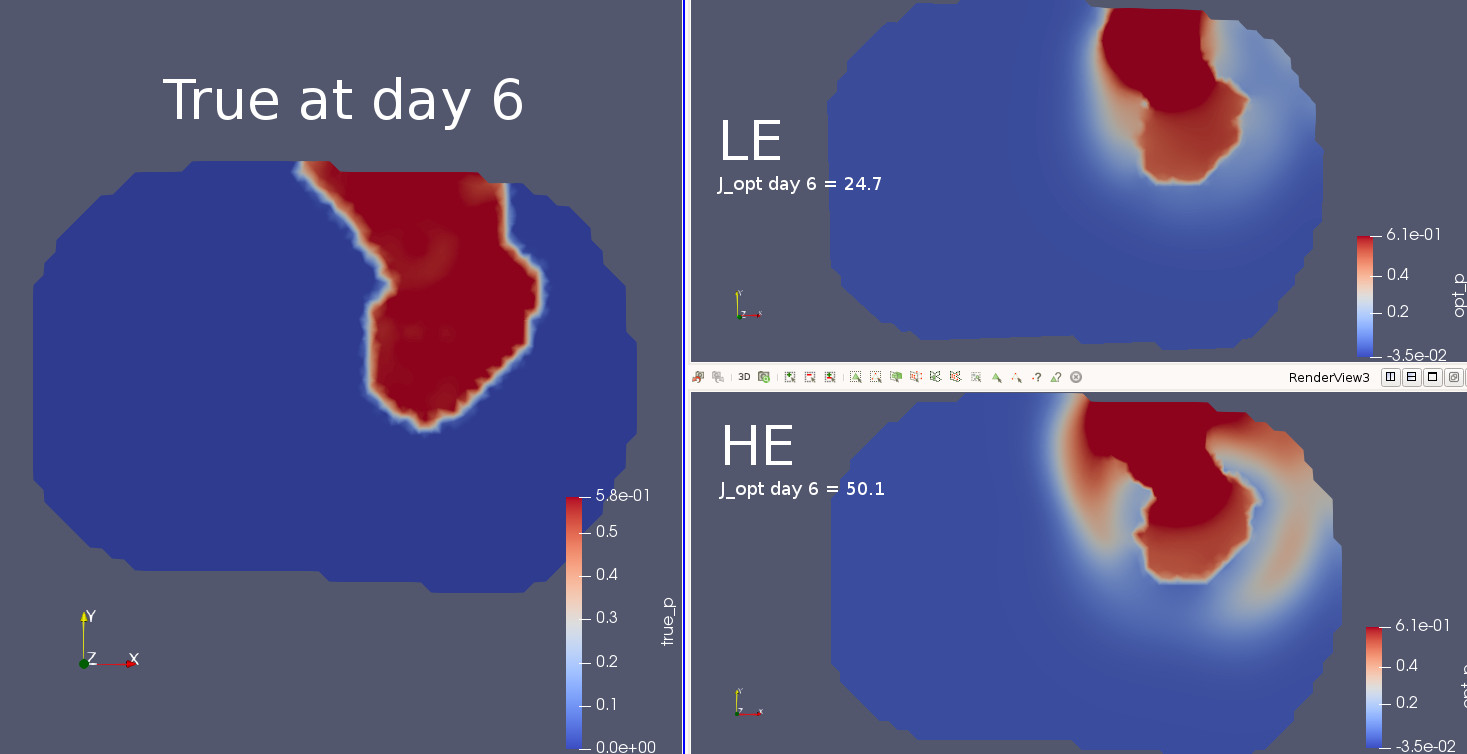
\includegraphics[width=\textwidth]{opt_day6.jpg}    	
    	\caption{Running the forward models to day 6 using parameter estimation results from forward model with day 2. LE performs better now.}
    	\end{figure}	
\end{frame}

\begin{frame}{Results: Forward to day 9}
	\begin{figure}
    	\centering
    	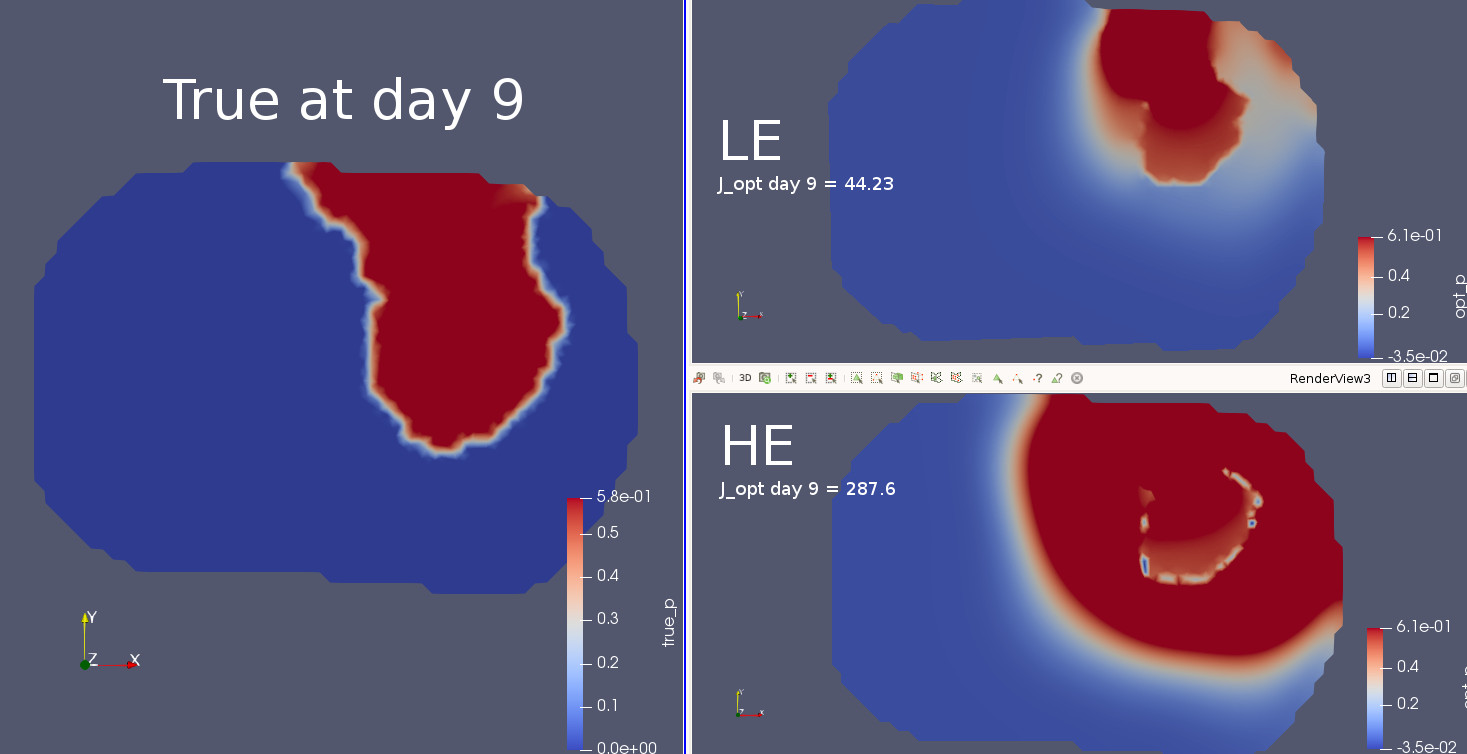
\includegraphics[width=\textwidth]{opt_day9.jpg}    	
    	\caption{Running the forward models to day 9 using parameter estimation results from forward model with day 2. LE performs better now.}
    	\end{figure}	
\end{frame}

There are some interesting differences here. It will be interesting to see what happens with varying $\beta$ values set for both of them. 
\begin{frame}{To do/try}
	\begin{minipage}[T][.7\textheight][t]{\textwidth}
		\begin{itemize}
			\item I am looking to add regularization to k next, 
			\[ r_1||k||^2 + r_2||\nabla k||^2\]
			\item I believe David used $\beta$ = 1 so I will try this as well. 
		\end{itemize}
	\end{minipage}
\end{frame}



%===============================================================================
% SLIDE 01
\section{Data for Fenics}
\subsection{Total Growth}
%===============================================================================

%\begin{frame}{Comparisons of Tumor Growth Between Rats}
%	\begin{minipage}[T][.7\textheight][t]{\textwidth}
%		\begin{figure}
%    	\centering
%    	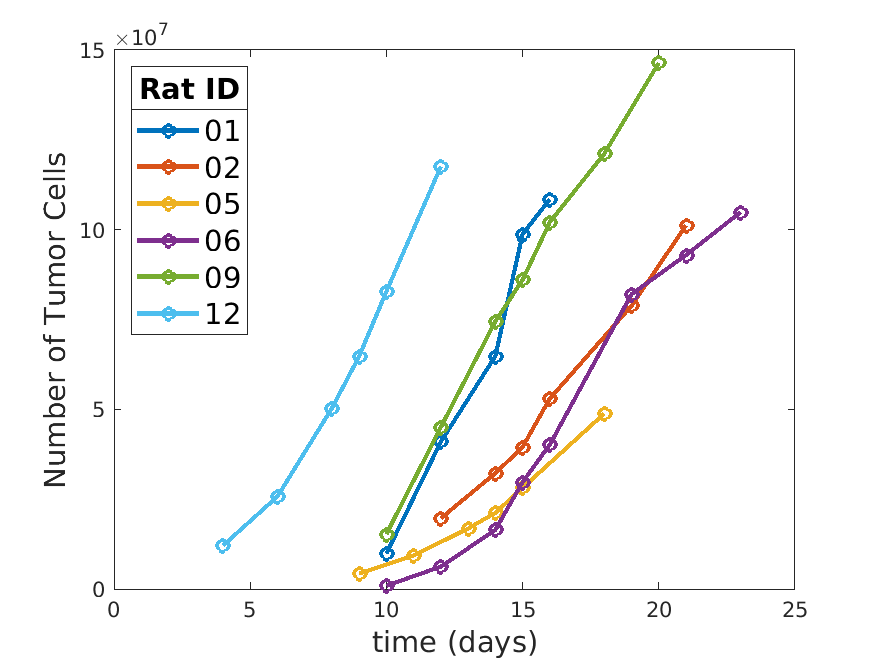
\includegraphics[width=.45\textwidth]{../../mouse-data/images/numtumorcells.png}    	
%    	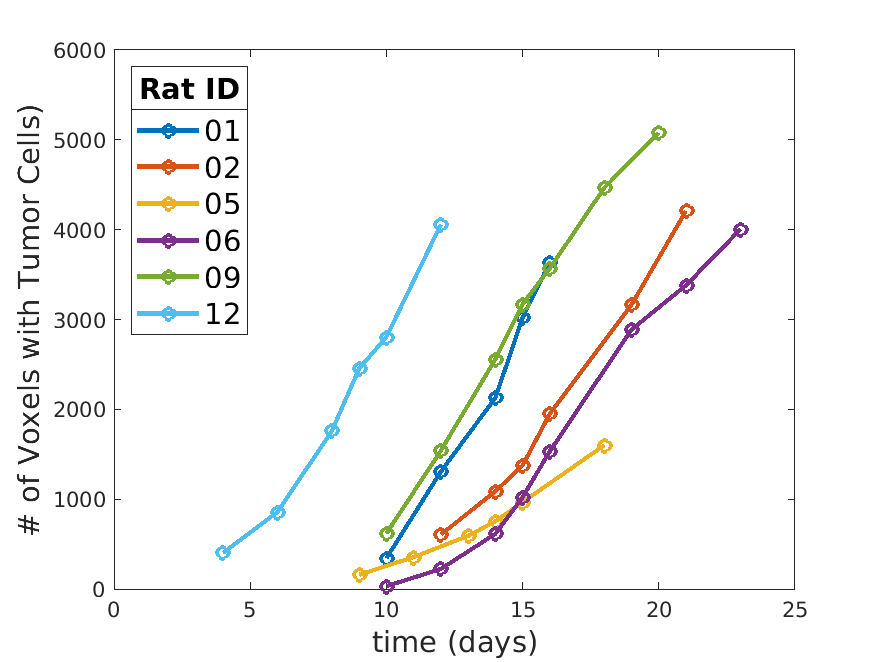
\includegraphics[width=.45\textwidth]{../../mouse-data/images/voxtumorcells.png}
%    	\caption{Tumor growth over time in different rats. \textbf{Left:} Cellularity (total measured number of tumor cells). \textbf{Right:} Number of voxels (3D) that have a nonzero amount of tumor cells.}
%    	\end{figure}
%	\end{minipage}
%\end{frame}
%
%\begin{frame}{Comparisons of Tumor Growth Between Rats}
%	\begin{minipage}[T][.7\textheight][t]{\textwidth}
%		\begin{figure}
%    	\centering
%    	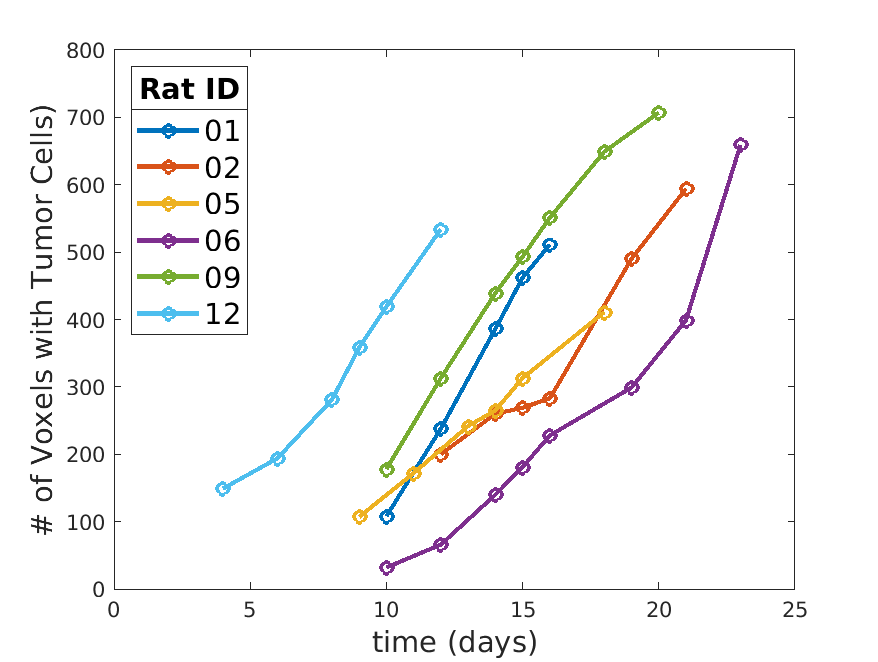
\includegraphics[width=.45\textwidth]{../../mouse-data/images/areatumorcells.png}    	
%    	\caption{Number of pixels (2D) with tumor cells in the slice that had the most initial tumor cells for each rat.}
%    	\end{figure}
%	\end{minipage}
%\end{frame}



\end{document}
